\documentclass[9pt,landscape,a4paper]{extarticle}
\usepackage[utf8]{inputenc}
\usepackage[ngerman]{babel}
\usepackage{tikz}
\usetikzlibrary{shapes,positioning,arrows,fit,calc,graphs,graphs.standard}
\usepackage[nosf]{kpfonts}
\usepackage[t1]{sourcesanspro}
%\usepackage[lf]{MyriadPro}
%\usepackage[lf,minionint]{MinionPro}
\usepackage{multicol}
\usepackage{wrapfig}
\usepackage[top=0.2mm,bottom=1mm,left=1mm,right=1mm]{geometry}
\usepackage[framemethod=tikz]{mdframed}
\usepackage{microtype}
\usepackage{bbold}
\usepackage{wrapfig}
\usepackage{amsmath} % to get \tfrac
% and to redefine some commands:
\let\oldforall\forall
\let\forall\undefined
\DeclareMathOperator{\forall}{\oldforall}

\usepackage{xfrac} % to get \sfrac
\usepackage{dsfont} % For mathbb{1}

% START CHEATSHEET TEMPLATE

\usepackage[default]{raleway}
\usepackage{fontawesome}
\usepackage[T1]{fontenc}

\usepackage{hyperref}
\usepackage{enumitem}
\setlist[enumerate]{itemsep=0mm}
\usepackage{lipsum}

\usepackage{xcolor}
\definecolor{customcolor}{HTML}{b5e9ff}
\definecolor{alert}{HTML}{CD5C5C}
\definecolor{w3schools}{HTML}{4CAF50}
\definecolor{subbox}{gray}{0.60}
\definecolor{codecolor}{HTML}{000000}
\colorlet{xx}{customcolor}

\usepackage{paralist}

% custom commands for typsetting
\newcommand{\Prob}[0]{\mathbb{P}}
\newcommand{\Quob}[0]{\mathbb{Q}}
\newcommand{\Ex}[0]{\mathbb{E}}
\newcommand{\Var}[0]{\textup{Var}}
\newcommand{\argmin}[0]{\textup{argmin}}
\newcommand{\se}[0]{\textup{se}}

%--------------------------Editor mode.

\usepackage
[citestyle=authoryear,
sorting=nty,	  		%Sorts bibliography by year, name, title
autocite=footnote, 		%Autocite command generates footnotes
autolang=hyphen, 		
mincrossrefs=1, 	
backend=biber]
{biblatex}

\DeclareFieldFormat{postnote}{#1}
\DeclareFieldFormat{multipostnote}{#1}
\DeclareAutoCiteCommand{footnote}[f]{\footcite}{\footcites}

\bibliography{literature}
% ----------------------------------------
% --------------------------------------------------------------------------------
\usepackage{tcolorbox}

\tcbuselibrary{most,listingsutf8,minted}

\tcbset{tcbox width=auto,left=1mm,top=1mm,bottom=1mm,
right=1mm,boxsep=1mm,middle=1pt}

\newenvironment{mycolorbox}[2]{%
\begin{tcolorbox}[grow to left by=-1em,grow to right by=-1em,capture=minipage,fonttitle=\large\bfseries, enhanced jigsaw,boxsep=1mm,colback=#1!30!white,on line,tcbox width=auto, toptitle=0mm,colframe=#1,opacityback=0.7,nobeforeafter,title=#2]%
}{\end{tcolorbox}\\[0.2em]}

\newenvironment{subbox}[2]{%
\begin{tcolorbox}[capture=minipage,fonttitle=\normalsize\bfseries, enhanced jigsaw,boxsep=1mm,colback=#1!30!white,on line,tcbox width=auto,left=0.3em,top=1mm, toptitle=0mm,colframe=#1,opacityback=0.7,nobeforeafter,title=#2]\footnotesize %
}{\normalsize\end{tcolorbox}\vspace{0.1em}}

\newenvironment{multibox}[1]{%
\begin{tcbraster}[raster columns=#1,raster equal height,nobeforeafter,raster column skip=1em,raster left skip=1em,raster right skip=1em]}{\end{tcbraster}}

\newenvironment{textbox}[1]{\begin{mycolorbox}{customcolor}{#1}}{\end{mycolorbox}}

%-------------------------------
\newtcblisting{codebox}[2]{colback=white,colframe=codecolor!80!black,listing only, 
minted options={numbers=left,style=tcblatex,fontsize=\scriptsize,breaklines,autogobble,linenos=false,numbersep=1mm},enhanced,breakable,boxsep=0pt,right=0pt,
left*=0.5mm,top=0pt,bottom=0pt,beforeafter skip=1mm,grow to left by=.5mm,grow to right by=.5mm,
title=#2, fonttitle=\bfseries,
listing engine=minted,minted language=#1}

%--------------------------------------------------------------------------------
\newcommand{\punkti}{~\lbrack\dots\rbrack~}

\renewenvironment{quote}
               {\list{\faQuoteLeft\phantom{ }}{\rightmargin\leftmargin}%
                \item\relax\scriptsize\ignorespaces}
               {\unskip\unskip\phantom{xx}\faQuoteRight\endlist}
               

%--------------------------------------------------------------------------------
\newcommand{\bgupper}[3]{\colorbox{#1}{\color{#2}\huge\bfseries\MakeUppercase{#3}}}
\newcommand{\bg}[3]{\colorbox{#1}{\bfseries\color{#2}#3}}

\newcommand{\mycommand}[2]{{\ttfamily\detokenize{#1}}~\dotfill{}~{\footnotesize #2}\\}
\newcommand{\sep}{{\scriptsize~\faCircle{ }~}}


\newcommand{\bggreen}[1]{\medskip\bgupper{w3schools}{black}{#1}\\[0.5em]}
\newcommand{\green}[1]{\smallskip\bg{w3schools}{white}{#1}\\}
\newcommand{\red}[1]{\smallskip\bg{alert}{white}{#1}\\}

\usepackage{multicol}
\setlength{\columnsep}{4pt}

\setlength{\parindent}{0pt}
\pagestyle{empty}

\usepackage{csquotes}

\newcommand{\loremipsum}{Lorem ipsum dolor sit amet.}

% END CHEATSHEET TEMPLATE

\let\bar\overline

\definecolor{myblue}{cmyk}{1,.72,0,.38}
\definecolor{mygreen}{cmyk}{76, 0, 76, 0.2}

\def\firstcircle{(0,0) circle (1.5cm)}
\def\secondcircle{(0:2cm) circle (1.5cm)}

\colorlet{circle edge}{myblue}
\colorlet{circle area}{myblue!5}

\tikzset{filled/.style={fill=circle area, draw=circle edge, thick},
    outline/.style={draw=circle edge, thick}}

\pgfdeclarelayer{background}
\pgfsetlayers{background,main}

\everymath\expandafter{\the\everymath \color{myblue}}
\everydisplay\expandafter{\the\everydisplay \color{myblue}}

\renewcommand{\baselinestretch}{.8}
\pagestyle{empty}




\makeatletter
\renewcommand{\section}{\@startsection{section}{1}{0mm}%
                                {.2ex}%
                                {.2ex}%x
                                {\color{myblue}\sffamily\small\bfseries}}
\renewcommand{\subsection}{\@startsection{subsection}{1}{0mm}%
                                {.2ex}%
                                {.2ex}%x
                                {\color{mygreen}\sffamily\bfseries}}
\renewcommand{\subsubsection}{\@startsection{subsubsection}{1}{0mm}%
                                {.2ex}%
                                {.2ex}%x
                                {\sffamily\bfseries}}
\makeatother

\def\multi@column@out{%
   \ifnum\outputpenalty <-\@M
   \speci@ls \else
   \ifvoid\colbreak@box\else
     \mult@info\@ne{Re-adding forced
               break(s) for splitting}%
     \setbox\@cclv\vbox{%
        \unvbox\colbreak@box
        \penalty-\@Mv\unvbox\@cclv}%
   \fi
   \splittopskip\topskip
   \splitmaxdepth\maxdepth
   \dimen@\@colroom
   \divide\skip\footins\col@number
   \ifvoid\footins \else
      \leave@mult@footins
   \fi
   \let\ifshr@kingsaved\ifshr@king
   \ifvbox \@kludgeins
     \advance \dimen@ -\ht\@kludgeins
     \ifdim \wd\@kludgeins>\z@
        \shr@nkingtrue
     \fi
   \fi
   \process@cols\mult@gfirstbox{%
%%%%% START CHANGE
\ifnum\count@=\numexpr\mult@rightbox+2\relax
          \setbox\count@\vsplit\@cclv to \dimexpr \dimen@-1cm\relax
\setbox\count@\vbox to \dimen@{\vbox to 1cm{\header}\unvbox\count@\vss}%
\else
      \setbox\count@\vsplit\@cclv to \dimen@
\fi
%%%%% END CHANGE
            \set@keptmarks
            \setbox\count@
                 \vbox to\dimen@
                  {\unvbox\count@
                   \remove@discardable@items
                   \ifshr@nking\vfill\fi}%
           }%
   \setbox\mult@rightbox
       \vsplit\@cclv to\dimen@
   \set@keptmarks
   \setbox\mult@rightbox\vbox to\dimen@
          {\unvbox\mult@rightbox
           \remove@discardable@items
           \ifshr@nking\vfill\fi}%
   \let\ifshr@king\ifshr@kingsaved
   \ifvoid\@cclv \else
       \unvbox\@cclv
       \ifnum\outputpenalty=\@M
       \else
          \penalty\outputpenalty
       \fi
       \ifvoid\footins\else
         \PackageWarning{multicol}%
          {I moved some lines to
           the next page.\MessageBreak
           Footnotes on page
           \thepage\space might be wrong}%
       \fi
       \ifnum \c@tracingmulticols>\thr@@
                    \hrule\allowbreak \fi
   \fi
   \ifx\@empty\kept@firstmark
      \let\firstmark\kept@topmark
      \let\botmark\kept@topmark
   \else
      \let\firstmark\kept@firstmark
      \let\botmark\kept@botmark
   \fi
   \let\topmark\kept@topmark
   \mult@info\tw@
        {Use kept top mark:\MessageBreak
          \meaning\kept@topmark
         \MessageBreak
         Use kept first mark:\MessageBreak
          \meaning\kept@firstmark
        \MessageBreak
         Use kept bot mark:\MessageBreak
          \meaning\kept@botmark
        \MessageBreak
         Produce first mark:\MessageBreak
          \meaning\firstmark
        \MessageBreak
        Produce bot mark:\MessageBreak
          \meaning\botmark
         \@gobbletwo}%
   \setbox\@cclv\vbox{\unvbox\partial@page
                      \page@sofar}%
   \@makecol\@outputpage
     \global\let\kept@topmark\botmark
     \global\let\kept@firstmark\@empty
     \global\let\kept@botmark\@empty
     \mult@info\tw@
        {(Re)Init top mark:\MessageBreak
         \meaning\kept@topmark
         \@gobbletwo}%
   \global\@colroom\@colht
   \global \@mparbottom \z@
   \process@deferreds
   \@whilesw\if@fcolmade\fi{\@outputpage
      \global\@colroom\@colht
      \process@deferreds}%
   \mult@info\@ne
     {Colroom:\MessageBreak
      \the\@colht\space
              after float space removed
              = \the\@colroom \@gobble}%
    \set@mult@vsize \global
  \fi}
  
% https://tex.stackexchange.com/questions/43008/absolute-value-symbols
\usepackage{mathtools}

\DeclarePairedDelimiter\abs{\lvert}{\rvert}%
\DeclarePairedDelimiter\norm{\lVert}{\rVert}%

% Swap the definition of \abs* and \norm*, so that \abs
% and \norm resizes the size of the brackets, and the 
% starred version does not.
\makeatletter
\let\oldabs\abs
\def\abs{\@ifstar{\oldabs}{\oldabs*}}
%
\let\oldnorm\norm
\def\norm{\@ifstar{\oldnorm}{\oldnorm*}}

\makeatother
\setlength{\parindent}{0pt}

\begin{document}
\begin{multicols*}{4}
\scriptsize
A matrix $A$ is \textbf{positive definite} if $y^T A y > 0 \forall y \neq 0$.
Two vectors $d_i$ and $d_j$ are said to be \textbf{conjugate} with respect to a symmetric matrix $A$ if $d_i^T Ad_j = 0 \forall i \neq j$.
A function is \textbf{convex}: $f'>0$. $-f$ is concave iff $f$ is convex.
\section*{Introduction into Nonlinear Optimization}

\subsection*{Unconstrained Optimization}

\textbf{Problem definition}
Given a set $X\subset R^n$ and a function $f: X \rightarrow R$, determine a $x^* \in X$ with the properties $f(x^*) \leq f(x)$ $\forall x \in X$ for a global minimum and $\forall x$ near $x^*$ for a local minimum, resp.

Necessary and sufficient optimality conditions for a local min.: $\nabla f (x^*) = 0 \Leftrightarrow \norm{\nabla f(x^*)} = 0$, $\nabla^2 f(x*3)$ is positive definite.

\textbf{Rate iterative methods}
Asymptotic rate of convergence: $\lim_{k\to\infty} (\sfrac{\norm{x^{k+1} - x^*}}{\norm{x^k - x^*}^p}) = \epsilon$, where p is the asymptotic order and $\epsilon$ the asymptotic error.
Convergence tests: $\norm{x^{k+1}-x^k}<\epsilon$ and/or $\norm{\nabla f(x^{k+1})}<\epsilon$ for sufficiently large $k$ and small $\epsilon$.

\textbf{Steepest Descent}
Linear convergence. $x^{k+1} = x^{k} + d^k \min_{t \in R}(f(x^k + t d^k))$ with $d^k = -\nabla f(x^k)$.

\textbf{Conjugate Gradient (CG, PCG) methods}
No matrix-matrix mult, only vectors. Solve large systems of eqs. Works only for symmetric positive definite matrices.
$d^{k+1} = -\nabla f(x^{k+1}) + \beta^k d^k$. Search direction better than steepest descent, as there, the angle between search directions can be very small (close Zic-Zac). 
$\beta^k$ either: Plak Ribière: $\beta^k= \sfrac{\nabla f (x^k)^T (\nabla f(x^k) - \nabla f(x^{k-1}))}{\norm{\nabla f (x^{k-1})}^2}$ or Fletcher Reeves: $\beta^k= \sfrac{\norm{\nabla f(x^k)}^2}{\norm{\nabla f (x^{k-1})}^2}$.
Preconditioning (PCG): Cholesky. %\texttt{pcg, ichol, mchol}.

\textbf{Newton Method}
Quadratic convergence. 
Avoids the inversion of the Hessian-matrix by quadratic approximation of the function $f$. The linear system of equations $\nabla^2 f(x^k) d^{k} = -\nabla f(x^k) \Leftrightarrow d^k = - (\nabla^2 f(x^{k}))^{-1} \nabla f(x^k)$ (Newton-equation) is solved instead, to get $x^{k+1}=x^k + d^k$.
No guarantee that a solution exists at the current iteration point. Newton search direction is not necessary a descent direction.
Ensure local convergence by step size strategy and choosing the steepest descent as the search direction at the current iteration $\rightarrow$ descent search direction.

\textbf{Quasi-Newton Method}
Super-linear convergence. No linear system of equations are solved.
Approximate Hessian-Matrix $B^k$. 
Updating formula: Broyden, Fletcher, Goldfarb and Shanno (BFGS) and DFP.
Condition on update: \textit{secant equation}: $B^{k+1} (x^{ki+1}-x^{k}) =B^{k+1} s^{k}=y^{k}= \nabla f^{k+1}-\nabla f^{k}$. 
Displacement $s^k$ and change of gradients $y^k$ must satisfy \textit{curvature condition}, $(s^k)^Ty^k>0$ for symmetric positive definite matrix $B^{k+1}$ map $s^k$ into $y^k$.
Additional requirement for uniqueness: $\min_B(\norm{B-B^k}),$ with $B = B^T, Bs^k=y^k$. 
Different norms $\leftrightarrow$ different Quasi-Newton methods.
BFGS-Method: $B^{k+1} = B^{k} - \frac{B^k s^k (s^k)^T B^k}{(s^k)^T B^k s^k} + \frac{y^k (y^k)^T}{(y^k)^T s^k}$. % not subject of exam

\textbf{Gauss-Newton Method}
Also Q-N. 
Approximation of Newton Method for least squares problem: $\min_{x \in R^n}(f(x))= \frac{1}{2} \norm{F(x)}^2, F: R^n \rightarrow R^m, m \gg n$. 
Convergence rate highly dependent on approximation of Hessian and order of non-linearity of $f$. 
Searching direction by $\nabla f (x) = \nabla F(x)^T F(x)$ $\Rightarrow$ $d_{GN}^k = - (\nabla F(x^k)^T \nabla F(x^k))^{-1} (\nabla F(x^k)^T F(x^k))$

\textbf{Levenberg-Marquardt Method}
Also Q-N. 
Gauss-Newton fails for singular $\nabla F(x^k)^T \nabla F(x^k)$. LM fixes this with trust region radius $\Delta^k$: $\min_{x \in R^n}(f(x))= \frac{1}{2} \norm{F(x^k) + \nabla F(x^k) d^k}^2, \norm{x^k} \leq \Delta^k$. 
If this condition is not fulfilled, it is not equivalent anymore to the Gauss-Newton method, as of the introduction of parameter $\lambda > 0$: $ (\nabla F(x^k)^T \nabla F(x^k) + \lambda \mathbb{1}) d_{LM}^k = - \nabla F(x^k)^T F(x^k)$.

\subsection*{Constrained Optimisation}
Transform constrained problem to a sequence of unconstrained problems. 
Optimality condition not simply performing the first and the second derivative of the objective function anymore.

\textbf{Set of active constraints}: $A(x) = I_{eq} \cup \left\{ i \in I_{in} \mid c_i = 0 \right\}$ 
\textbf{Linear independence constrained qualification LICQ}: The set of active constrained gradients at the solution $\{ \nabla c_i (x^*), i \in A(x^*) \}$ is linearly independent.
\textbf{Feasible directions}: those vectors from the current point that locally satisfy the constraints.
\textbf{Lagrange formulation} of the optimization problem (with $\lambda_i$: Lagrange multiplier): $L(x,\lambda) = f(x) - \sum_{i\in A(x)}\lambda_i c_i (x)$.
\textbf{Critical cone}: $\kappa(x^*, \lambda^*) = \{d \in F(x^*) \mid \nabla c_i (x^*) ^T d = 0, \forall i \in A(x^*) \text{ with } \lambda_i^* > 0$.

\textbf{First order conditions} (for constrained problems): \textit{KKT-conditions}: $\nabla_x L(x^*, \lambda^*) = 0, c_i(x^*) = 0 \forall i \in I_{eq}, c_i (x^*) \geq 0 \forall i \in I_{in}, \lambda_i^* \geq 0 \forall i \in I_{in}, \lambda_o^* c_i (x^*) = 0 \forall i \in I_{eq} \cup I_{in}$. Gradient is $\nabla_x L (x, \lambda) = \nabla_x f(x) - \sum_{i\in A(x)} \lambda_i \nabla_x c_i (x)$

\textbf{Second order conditions} (for constrained problems): KKT-conditions as well as:
For weak local minimum: critical cone: $d^T \nabla_{xx}^2 L(x^* \lambda^*)d \geq 0 \forall d \in \kappa(x^*, \lambda^*)$.  
For strong local minimum: $d^T \nabla_{xx}^2 L(x^* \lambda^*)d > 0 \forall d \in \kappa(x^*, \lambda^*)$

\textbf{Penalty method}
Introduce penalty function: $P(x,a) = f(x) + \frac{\alpha}{2} \sum_i^p c_i^2 (x)$. Solve with $\alpha$ increasing.

\textbf{Sequential quadratic programming (SQP) Method}
One of the most effective for solving nonlinear (small and large) problems including highly nonlinear constraints.
Model the problem $\min_{x\in R^n} f(x), c_i (x) = 0 \forall i \in I_{eq}, c_i (x) \geq 0 \forall i \in I_{in}$ by a quadratic programming subproblem $min_{d \in R^n} (\frac{1}{2} d^T \nabla_xx^2 L (x^k, \lambda^k) d + \nabla f (x^k)^T d + f(x^k)), c_i (x^k) + \nabla c_i (x^k)^T d = 0 \forall i \in I_{eq}, c_i (x^k) + \nabla c_i (x^k)^T d \geq 0 \forall i \in I_{in}$ at each iterate and define the search direction $d$ as the solution of the subproblem.
The new constraints are linearizations of the original constraints
Note: $L(x,\lambda) = f(x) - \sum_{i\in A(x)}\lambda_i c_i (x)$
In constrained gradient based optimization problems, quadratic subproblems have often to be solved $\Rightarrow$ fix with:

\subsection*{Gradient-free methods}
\textbf{Genetic-Algorithms}
Simple, can find global minimum, require lots of function evaluations (but those only). A new generation of individuals is produced using crossover, mutation, ..., operations.

%\begin{wrapfigure}{R}{0.5\linewidth}
\begin{figure}[H]
    \vspace{-0.5cm}
    \centering
    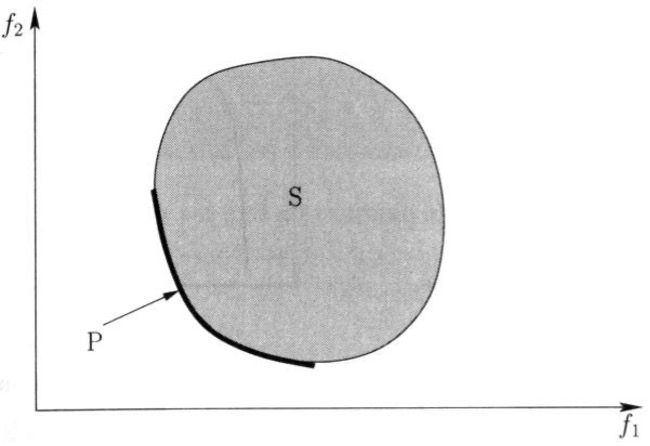
\includegraphics[width=0.4\linewidth]{img/pareto.jpg}
    \caption{\label{fig:pareto}Pareto front and set}
\end{figure}
\vspace{-0.5cm}
%\end{wrapfigure}

\subsection*{Multiobjective Optimization}
Tradeoff surface (Pareto front): $S$ is a set of values of pair ($f_1$, $f_2$) when x respects the constraints, $P$ is the tradeoff surface.
\textbf{Pareto optimal}: A design variable $x^* \in S$ and the corresponding $f(x^*)$ are pareto optimal if there does not exist another design variable $x\in S$ such that $f_i (x) \leq f_i (x^*) \forall i = 1 ... k$ and $f_j (x) < f_j (x^*)$ for at least one objective function $f_j$.


\subsubsection*{Solution methods}
\textbf{Scalar methods}: 
\textit{Weighted sum of objective functions} (only for convex sets $S$): transform problem into monoobjective as $f_{eq}(x) = \sum_{i=1}^k w_i \cdot f_i(x)$ with weights $w_i \geq 0, \sum_{i=1}^k w_i = 1$. 
\textit{Goal attainment method} 
Minimize $\lambda$ with $f_i (x) - w_i \cdot \lambda \leq F_i$ under the constraints. 
$F$ is an initial vector of ideal objective function values and $w$ the search direction/weights. 
The feasible set $S$ is not required to be convex.

% \textbf{Active-Set-Strategy} % not part of exam

\section*{Design of Experiments (DoE)}
\section*{Introduction into Nonlinear Finite Element Analysis}

From continuum: $\div{\sigma} + b = 0, u_s = \bar{u} \text{ on } \partial\Omega_u, \sigma \cdot n = t = \bar{t} \text{ on } \partial\Omega_t$
to a discrete system: $K\hat{u}=f$ (linear FEM) and $K\Delta \hat{u} = \Delta f$ (nonlinear).
isoparametric concept: 
The geometry as well as the displacements field is approximated with the same shape functions.
$\hat{u}$: nodal displacements. $N$: matrix of interpolation functions. $B$: strain displacement matrix.
Mapping from isoparametric space to real space by Jacobi $J^{-1}$.

\textbf{4-Node bilinear element}
has shape/interpolation functions, $N_1 = \sfrac{1}{4}(1-r)(1-s), N_2 = \sfrac{1}{4}(1+r)(1-s), N_3 = \sfrac{1}{4}(1+r)(1+s), N_4 = \sfrac{1}{4}(1-r)(1+s)$, interpolation matrix $N=
\begin{bmatrix}
N_1 & 0 & N_2 & 0 & N_3 & 0 & N_4 & 0 \\
0 & N_1 & 0 & N_2 & 0 & N_3 & 0 & N_4
\end{bmatrix}$, nodal displacements $\hat{u} = \begin{bmatrix}
\hat{u}_x^{(1)} & \hat{u}_y^{(1)} & \hat{u}_x^{(2)} & \hat{u}_y^{(2)} &
\hat{u}_x^{(3)} & \hat{u}_y^{(3)} & \hat{u}_x^{(4)} & \hat{u}_y^{(4)}
\end{bmatrix}$ and strain interpolation matrix $B_i = \begin{bmatrix}
\sfrac{\partial N_i}{\partial x} & 0 \\
0 & \sfrac{\partial N_i}{\partial y} \\
\sfrac{\partial N_i}{\partial y} & \sfrac{\partial N_i}{\partial x} \\
\end{bmatrix}$, $B= \begin{bmatrix}
B_1 & B_2 & B_3 & B_4
\end{bmatrix}$, $J^{-1}\begin{bmatrix}
\sfrac{\partial N_i}{\partial r} \\
\sfrac{\partial N_i}{\partial s}
\end{bmatrix} =\begin{bmatrix}
\sfrac{\partial N_i}{\partial x} \\
\sfrac{\partial N_i}{\partial y}
\end{bmatrix}$.

Element force vectors are given by
$f_e^{int} = \int_{\Omega^e} B^T \sigma dV$, $f_e^{ext} = \int_{\Omega^e} N^T b  dV + \int_{\partial\Omega^e} N^T t  da$.
Using numerical integration, that is $f_e^{int} = \sum_{i=1}^{n_{\text{gaussp}}} w_i B_i ^T \sigma_i \det{J_i}$ and $f_e^{ext} = \sum_{i=1}^{n_{\text{gaussp}}} w_i N_i ^T b_i \det{J_i} + \sum_{i=1}^{n_{\text{gaussp}}} w_i^b N_i ^T t_i \sigma_i \det{J_i^b}$, respectively.

Assemble globally: $f^{int} = \bigcup_{e=1}^{n_{\text{elem}}} f_e^{int}$,  $f^{ext} = \bigcup_{e=1}^{n_{\text{elem}}} f_e^{ext}$ ($\bigcup$: finite element assembly operator).

For linear elasticity, we have the elasticity matrix $D^e$ related as $\sigma= D^e \epsilon = D^e B \hat{u}$, and the stiffness matrix $K ^e = \int_{\Omega^e} B^T D^e B dV$.

\textbf{Nonlinear FEM}
Material tensor $D$ is not constant. Iteration of Newton scheme requires solving $K \delta \hat{u}^{(k)} = r^{(k-1)}$ for $\delta \hat{u}^{(k)}$.
$r^{(k-1)}$ are the residual forces.
Update the global displacements as $\hat{u}_{n+1}^{(k)} = \hat{u}_{n+1}^{(k-1)} + \delta \hat{u}^{(k)}$.

\subsection*{Constrained Optimization in FEM}
\textbf{Contact Modelling (Imposition of Constraints)}
\textit{Penalty Method:}
The potential energy of a discretized system is given by $\Pi = \sfrac{1}{2} U^T K U - U^T R$ with $U\in\doubleR^n$: nodal displacements, $K\in\doubleR^{n\times n}$: global stiffness matrix and $R\in\doubleR^n$: external forces on nodes.
First term: elastic, second: potential (of external forces) energy.
Boundary conditions: $ZU=V$, $Z\in\doubleR^{m \times n}, V\in \doubleR^m$, $m$: Nr. of boundary conditions. 
Add the violation as a penalty term:
$\Pi = \sfrac{1}{2} U^T K U - U^T R + \sfrac{\alpha}{2}(ZU-V)^T(ZU-V)$.
Choose $\alpha \gg K_{?,?}$.
To minimize: $\partial\Pi = \partial U^T (KU -R+\alpha Z^T (ZU-V))=0$.
Has to be fulfilled for every $\partial U^T \Rightarrow U = (K+\alpha Z^T Z)^{-1} (R+\alpha Z^T V)$

\textit{Lagrange Multiplier Method:}
$\Pi = \sfrac{1}{2} U^T K U - U^T R + \lambda^T (ZU-V)$, and with $\partial \Pi = 0$, we get $\begin{bmatrix}
K & Z^T \\
Z & 0
\end{bmatrix} \begin{bmatrix}
U \\
\lambda
\end{bmatrix} = \begin{bmatrix}
R \\
V
\end{bmatrix}$.
Where $\lambda$ is a vector of $m$ Lagrange multipliers.
Disadvantages: Bigger bandwidth $\rightarrow$ loss of $K$ typical band structure. The system matrix is symmetric but not positive definite.
\section*{Optimization based on Meta Modeling Techniques}
Metamodels tend to reduce the computational time significantly.

\textbf{Response Surface Method (RSM)}
Fit a surface to discrete points. Use the constructed function (meta-model) to solve the optimization (sub)problem.
Advantages: Tendency to approximate the global minimum. Avoids local outliers \& oscillations of the response thanks to smoothing. 
Optimization of RS leads to simple computations. 
Disadvantages: Efficient computations are restricted to a small number of variables (ca. 15).

\textbf{Error analysis}
Coefficient of determination:
$R^2 = \frac{\sum_{i=1}^{n_p} (\hat{y}_i-\bar{y})^2}{\sum_{i=1}^{n_p} (y_i-\bar{y})^2}$
with $n_p$: number of exp. points, $y_i$: actual response, $\hat{y}_i$: predicted response, $\bar{y}$: mean values of responses.
$0\leq R^2 \leq 1$. $R^2=1$ indicates perfect fit.
Small $R^2$: the region of interest is too large or too small.
Overfitting possible. 
$R^2$ represents the ability of the response surface to predict the variation of the true response.

\textbf{Successive Response Surface Method (SRSM)}
Adapt the subdesign space.

\textbf{Kriging}
High quality approximation, very flexible models. 

Meta-model $y=f(x)+Z(x)$, with $y(x)$: unknown interest, $f(x)$: known polynomial, regression coefficient $a$, $Z(x)$: stochastic component with mean zero and $\cov{[Z(x^i), Z(x^j)]} = \sigma^2 R[R(x^i, x^j)]$, with $R$: $n\times n$ correlation matrix (symmetric, unit diagonal) with $R(x^i, x^j)$ correlation between $x^i, x^j$.
E.g. exponential: $R=\prod_{k=1}^{m}\exp{-\theta_k \abs{d_k}}$ or Gaussian: $R=\prod_{k=1}^{m}\exp{-\theta_k \abs{d_k^2}}$ with $m$: number of variables, $d_k=x_k^i - x_k ^j$.
$a, \sigma, \theta$ are unknown and depend on each other. 
Iterative procedure required!
An appropriate combination of the regression model and the stochasitc model as well as the number and the distribution of the sampling points is of crucial importance.
In general, the computational time of the fitting process is larger than using RSM.

\textbf{Validation (Cross-Validation) of the Meta-model}
1. Remove sample $x_i$ from the data set.
2. Evaluate the model for the remaining $n_p - 1$ samples.
3. Evaluate the model on the removed sample $x_i \rightarrow \hat{y}_{-1}$.
4. Repeat the points 1. – 3. for each point of the data set.
5. Compare the computed values with the data points of the real supporting points.
$\epsilon_{RMS}=\sqrt{\frac{1}{n_p} \sum_{i=1}^{n_p} (y_i-\hat{y}_{-i})^2}$.



\section*{Shape and Topology Optimization}
Discretize Geometry (CAGD) for the design model and mechanical model (FEM) for the analysis model to formulate the optimization problem. 

\textbf{SIMP-Approach for Continuous Material Topology Optimization}
SIMP = “Solid Isotropic Microstructure with Penalty for intermediate density”. 

\textbf{Analytical sensitivity analysis (computation of derivatives)}
Consider the linear FEM equations for the compliance problem:
$c(\rho_e) = u^T (\cup_{e=1}^{N}\rho_e^p K_e) u$,
$\min_{\rho_e} c(\rho_e)$, 
$\sum_{e=1}^N v_e \rho_e \leq V$, 
$0 < \rho_{\text{min}}\leq \rho_e \leq 1$, 
$e=1,...N$ (e: element, V: volume).
The derivative of the compliance is of the particularly simple form (at the element level):
$\sfrac{\partial c}{\partial \rho_e} = -p \rho_e^{p-1} u^T K_e u$.
Computation of the derivative of the objective function with respect to the design variables is required, if a gradient-based optimization method is applied!

\textbf{Filtering the sensitivities (numerical stabilization)}
Filtering of the sensitivity information is an efficient way to ensure mesh independency. 
This means: modifying the design sensitivity of a specific element, based on the weighted average of the
element sensitivities in a fixed neighborhood.
$\rightarrow$ no extra constraints need to be considered (very simple to implement)
$\sfrac{\hat{\partial c}}{\partial \rho_k} = \sfrac{1}{\rho_k \sum_{i=1}^N \hat{H_i}} \sum_{i=1}^N \hat{H_i} \rho_i \sfrac{\partial c}{\partial \rho_i}$.

The mesh independent factor $\hat{H_i}$ is written as
$\hat{H_i} = r_{\text{min}} - \text{dist}(k,i), \{i \in N | \text{dist}(k,i) \leq r_{\text{min}}\}$, 
$k = 1,...,N$ with $\text{dist}(k,i)$: distance between the center of element $k$ and element $i$.

\subsection*{Shape Optimization}
Determine the optimal shape of edges and surfaces. No change in topology.
Transformation of the variational problem into a parameter optimization problem
$\rightarrow$ Optimization variables $s$: free, discrete parameters which describe the shape of the structure.

\textbf{FE-node based approach}:
FE-nodes are directly defined as design variables.
Most freedom of shape change, no time-consuming shape parametrization process is required.
Either without filtering/smoothing techniques: lacks a length scale control that is necessary to ensure a well-posed shape optimization problem and avoid numerical instability, 
or with: motivated by the success of filtering techniques that impose minimum length scales in topology optimization.

\textbf{Computer Aided Geometric Design (CAGD) – based approach}
Design Elements (Splines, B-Splines, Bézier-Splines,....). Much less design variable than FE-node based.
Approximate geometry of the structure piecewise using so-called design elements (curves, surface, or volume elements).
Optimization variable: Position of the control points of the design elements. 
In general, the FE-mesh is much finer than the discretization with design elements. 
Because of the strict separation between the geometry model and analysis model, numerical instabilities are avoided.
Optimized shape is available in CAD format. 
Disadvantages:
Couplings between the CAGD model and the FE-model have to be supported by the program.
Problems due to re-meshing or definition of the new CAD model can occur.


\section*{Robustness and Sensitivity Analysis}

\subsection*{Robust Design Optimization (RDO)}
Robust Design Optimization methods determine an optimal design which is insensitive to uncertainties in certain design parameters.
FEM based optimization techniques can also directly be applied to RDO
In addition to the Design Variables (DV) in deterministic optimization, also Noise Variables (NV) come in to the picture, which have to be appropriately treated from the point of view of DoE and RSM.

Deterministic optimization will look for the optimal $\vec{x}^*$ which minimizes the objective function without taking the scatter into consideration!
The objective of the Robust Design (RD) optimization is to find a design with a minimal variance of the scattering model responses around the mean values of the design parameters
Optimized designs within the sigma level $\pm 2$ ($\pm 2\sigma = 95.4\%$) are characterized as Robust Design.

\textbf{Principle of nonlinearity}:
Assume the function $y$ is defined as: $y=f(\vec{x}, \vec{z})$. where $\vec{x}$ is the vector of design variables and $\vec{z}$ is the vector of noise variables. 
If we select values for our design variables $\vec{x}$ which minimize the so-called sensitivity coefficients $\sfrac{\partial f(\vec{x}, \vec{z})}{\partial z_i}$ we can also minimize the scatter of the outcome.

\textbf{Objective Functions for Robust Optimization}:
E.g., minimization of mean response ($\min(\mu_f - m)^2$, s.t. $\mu_f + k\sigma_f \leq USL, \mu_f - k\sigma_f \geq LSL$), minimization of standard deviation ($\min(\sigma_f)$, s.t. dito) or minimization of both ($\min(\mu_f - m)^2 + k \sigma_f^2$, s.t. dito).
USL = Upper Specification Limit.


\textbf{Single Response Surface Method}:
Robust Design Optimization based on Design of Experiments (DoE) and Response Surface Methods (RSM, SRSM)

The parameter set is now composed of the union of the DV’s and NV’s which are used in the DoE indistinctly.
The response surface is then fitted to the combined set of DV’s and NV’s directly: $y=f(\vec{x}, \vec{y})$.
The mean and variance functions are derived from this model, 
$\mu_y = E[f(\vec{x},\vec{z})]$ and $\sigma_y = Var[f(\vec{x},\vec{z})]^{\sfrac{1}{2}}$.
The DV’s and NV’s are included in the DoE in a mixed manner, thus substantial savings in computational cost can be made.
\section*{Fundamentals of Machine Learning}
SUPERVISED LEARNING: Develop a predictive model based on both input and output data.
UNSUPERVISED LEARNING: Discover an internal representation from input data only.

Main challenges: underfitting and overfitting (bias/variance tradeoff).
Overfitting happens when the model is too complex relative to the amount and noisiness of the training data. The possible solutions are: To simplify the model by selecting the one with fewer parameters (e.g., a linear model rather than a high-degree polynomial model),
or to gather more training data,
or to reduce the noise in the training data (e.g., fix data errors and remove outliers).
Constraining a model to make it simpler and reduce the risk of overfitting is called regularization.

\textbf{Regularization}
reduces the risk of overfitting.
Regularization forces the model to have a smaller slope, which fits a bit less the training data that the model was trained on, but actually allows it to generalize better to new examples.
The amount of regularization to apply during learning can be controlled by a hyperparameter. 
A hyperparameter is a parameter of a learning algorithm (not of the model).
Tuning hyperparameters is an important part of building a Machine Learning system.

\textbf{Testing and Validating}
The only way to know how well a model will generalize to new cases is to actually try it out on new cases. Therefore, split your data into two sets:
the training set and the test set. As these names imply, you train your model using the training set, and you test it using the test set.
The error rate on new cases is called the generalization error (or out-of-sample error), and by evaluating your model on the test set, you get an estimate of this error.
This value tells you how well your model will perform on instances it has never seen before.
If the training error is low but the generalization error is high, it means that your model is
overfitting the training data.
It is common to use 80\% of the data for training and hold out 20\% for testing.

Cross-validation can be applied to get an estimate of a model’s generalization performance.
If a model performs well on the training data but generalizes poorly according to the cross-validation metrics, then
your model is overfitting.
If it performs poorly on both, then it is underfitting. This is one way to tell when a model is too simple or too
complex.
Another way is to look at the learning curves: these are plots of the model’s performance on the training set and the validation set as a function of the training set size.

\textbf{Feature Scaling}
One of the most important transformations you need to apply to your data is feature scaling. With a few exceptions, Machine Learning algorithms don’t perform well when the input numerical attributes have very different scales.
There are two common ways to get all attributes to have the same scale: min-max (normalization, values are shifted and rescaled so that they end up ranging from 0 to 1 by subtracting the min value and dividing by the max minus the min.) scaling and standardization (First it subtracts the mean value (so standardized values always have a zero mean), and then it divides by the standard deviation so that the resulting distribution has unit variance.
Unlike min-max scaling, standardization does not bound values to a specific range, which may be a problem for some algorithms
Standardization is much less affected by outliers.).

\textbf{Linear Regression}
A linear model makes prediction by simply computing a weighted sum of the input featers, plus a constant called the bias term.
$\hat{y}=w^T x$.
Cost function: mean square error $MSE=\frac{1}{m} \sum_{i=1}^{m} (w^T x^i - y^i)^2$.

\textbf{Ridge- and Lasso Regression}
A good way to reduce overfitting is to regularize the model (i.e. to constrain it): The fewer degrees of freedom it has, the harder it will be for it to overfit the data.
The hyperparameter $\alpha$ controls how much you want to regularize the model.
Ridge Regression cost function: $J(w) = \frac{1}{m} \sum_{i=1}^{m} (w^T x^i - y^i)^2 + \frac{\alpha}{2} \sum_{i=1}^{m} w_i^2$.
Lasso Regression cost function: $J(w) = \frac{1}{m} \sum_{i=1}^{m} (w^T x^i - y^i)^2 + \alpha \sum_{i=1}^{m} \abs{w_i}$
\section*{Methods for Regression and Classification}

\textbf{Support Vector Machines} (SVM) 
can be used for classification or continuous values for regression. 
The class of an unseen data point is determined by comparing it with the support vectors in the training set by using the chosen kernel.
SVMs rely on solving a convex optimization problem.

\textit{Kernels}
define a hyperplane in a higher dimensional feature space where the data is linearly separable. 
The mapping to the higher dimensional space is defined by $\phi(x)$. 
Kernel functions calculate the similarity of the two vectors without having to calculate the mapping function $k(x,x')=\phi(x^T)\phi(x')$.
Common kernel functions:
Linear: $k(x,x') = x^T x'$, polynomial: $k(x,x')=(x^T x' + 1)^p, p\in\doubleN$, Gaussian: $k(x,x')=\exp{(-\sfrac{\norm{x-x'}^2}{2\sigma^2})}$, radial basis function: $k(x,x')=\exp{-\gamma\norm{x-x'}^2}$ (hyperparameter $\gamma$ determines how much influence data points with lower similarity have on the decision boundary).

\textbf{Support Vector Classification} (SVC):
In two-class classification, the goal is to find a decision surface $y(x)=w^T\phi(x)+b$, with $w$: learning parameter vector, $\phi(x)$: feature transformation, $b$: bias.
The training set consists of input samples $x_1,...x_N$ with corresponding target values $t_1,...,t_N$ where $t_i\in {-1,1}$.
Under the assumption that the data set is linearly separable in the transformed feature space $\phi(x)$, at least one solution $w,b$ exists such that $t_n y(x_n)>0$ for all data points.
SVMs find the single decision boundary $y(x)$ that maximizes the smallest distance between any sample to itself (also called the margin).

SVC is helpful, as the class of an unseen data point is determined by comparing it to the support vectors in the training set by using the chosen kernel.
The kernel trick allows for the insertion of an arbitrary kernel that corresponds to an indefinitely dimensional feature transformation (e.g., the Gaussian kernel), but without calculating the feature transformation.

\textit{Hard Margin SVC}: can lack from overfitting to the training data. In general, a perfect classification!
However, the resulting decision surface will give a poor generalization.

\textit{Soft Margin SVC}
A soft-margin SVC counteracts overfitting.
The approach of the hard-margin SVC is modified such that data points are allowed on the wrong side of the margin.
Slack variables $\xi_n$ are defined for every training data point: $\xi_n = \abs{t_n-y(x_n)}$.
A penalty is introduced that increases linearly with the distance from the boundary when a data point is misclassified.
With $C$ controlling trade-off between the slack variable penalty and the decision boundary: $\min(\frac{1}{2}\norm{w}^2)+C\sum_{n=1}^{N} \xi_n$, s.t. $t_n y(x_n) \geq 1 - \xi_n, n = 1,..., N$.

\textbf{Tipps \& Tricks}
Use FE results as training data for SVM classification.
Sample data points using Sliced Latin Hypercube Sampling. Filter out infeasible configurations.
Assess the performance of the SVM using Cross-Validation.

Hyperparameter optimization: Choose manually (difficult \& time consuming) or use an optimization process, e.g.:
\textit{SVM Optimization Equation with \textcolor{purple}{RBF Kernel}}: $\max_w (\Tilde{L}(w)) = \sum_{n=1}^N \lambda_n - \frac{1}{2} \sum_{n=1}^N \sum_{m=1}^N \lambda_n \lambda_m t_n t_m \textcolor{purple}{\exp{(-\gamma\norm{x_n-x_m}^2)}}$, with $\gamma$: kernel scale and $C$: box constraint, s.t. $0\leq \lambda_n \leq C, \sum_{n=1}^N \lambda_n t_n = 0$.

\textbf{K-Fold cross validation} 
separates the training data multiple times during the loss calculation to avoid introducing bias into the loss prediction.
There exist several classification loss equations.

\textbf{Kriging vs. SVM parameter determination}
Iterate until convergence. 
Kriging minimizes the cost function $L(\theta,sigma^2, a)$ for constant regression parameter $a$ to get $\theta, \sigma^2$. 
Thereafter, you minimize the cost function for constant correlation parameters $\theta$ and covariance $\sigma^2$ to get $a$. Start again.
For SVM, the cost function is $L(C, \gamma, w)$, first for constant $w$, then for constant hyper-parameters $C$ and $\gamma$.

\textbf{Support Vector Machines Regression} (SVR)
SVM not only does support linear and nonlinear classification, but it also supports linear and nonlinear regression.
Just reverse the objective: instead of trying to fit the largest possible street between two classes while limiting margin violations, SVM Regression tries to fit as many instances as possible on the street while limiting margin violations.
The width of the street is controlled by a hyperparameter $\epsilon$.
In SVR, the error function from Ridge Regression is replaced by a function that only penalizes data points that lie ouside the $\epsilon$-tube:

$E_\epsilon (t-y(x)) = \begin{cases} 
0 &\mbox{if } \abs{t-y(x)} < \epsilon \\
\abs{t-y(x)} - \epsilon & \mbox{otherwise}
\end{cases}$.
The regularized error function in SVR that needs to be minized is:
$\frac{1}{2} \norm{w}^2 - C \sum_{n=1}^N E_{\epsilon} (y(x_n) - t_n)$.
Note: $C$: Regularization parameter (hyper-parameter), $y(x_n)=w^T \phi(x_n)+b$.

Similar to SVC slack variables are introduced: $\xi$ and $\hat{\xi}$, per data point that needs to be optimized.
$\xi>0$ corresponds to a point that fulfils $t_n > y(x_n) + \epsilon$. 
$\hat{\xi}>0$ corresponds to a point that fulfils $t_n < y(x_n) - \epsilon$. 
The conditions on data points are: $t_n \leq y(x_n) + \epsilon + \xi_n$ and $t_n \geq y(x_n) - \epsilon - \hat{\xi}_n$.
Minimizing the slack variables leads to error function:
$\frac{1}{2} \norm{w}^2 - C \sum_{n=1}^N (\xi_n + \hat{\xi}_n)$, s.t. $\xi_n\geq 0, \hat{\xi}_n \geq 0$ and the said conditions on data points.

The dual formulation is found by substituting $y(x)$ and setting the derivatives of the Lagrangian to zero to be:
$max_{a_n, \hat{a}_n} \tilde{L} = \frac{1}{2} \sum_{n=1}^N \sum_{m=1}^N (a_n - \hat{a}_n) (a_m - \hat{a}_m) \textcolor{purple}{k(x_n,x_m)} - \epsilon \sum_{n=1}^N (a_n - \hat{a}_n) + \sum_{n=1}^N (a_n - \hat{a}_n)t_n$, 
s.t. $0\leq a_n \leq C, 0 \leq \hat{a}_n \leq C$.
Predictions for new inputs are made by $y(x) = \sum_{n=1}^N (a_n - \hat{a}_n) \textcolor{purple}{k(x,x_n)} + b$.

\textbf{Pricipal Component Analyis (PCA)}
Sampling covariance matrix of $X$ ($d$ features as columns, $n$ observations in rows): $C_X = \sfrac{1}{n-1}X^T X$.
Symmetric. Variance of the columns of $X$ in diagonal and correlation in off-diagonals.
Goal of PCA: find a coordinate system where $C_x = P^T C_Z P$ is diagonal. 
Columns of $P$ contain the eigenvectors of $C_X$, $C_Z$ is the sampling covariance with respect to the new basis $P$.
The new basis vectors are referred to as principal component directions.
$C_Z$ is diagonal and contains the variances of $Z = XP$.
The columns of $Z$ are called principal components.
Since the off-diagonal elements of $C_Z$ are zero, the correlations of the principal components are zero.
The dimensionality of $Z$ can be reduced by neglecting the principal components, which contribute the fewest of all to the total variance in the data.


\section*{Supervised and unsupervised learning}
\end{multicols*}
\end{document}
